\documentclass{llncs}


\usepackage[ngerman]{babel}
\usepackage[utf8]{inputenc}					%Mathe Befehle
\usepackage{amsmath}							%Mathe Features
\usepackage{amssymb}							%Mathe Sonderzeichen
\usepackage{stmaryrd}
\usepackage[usenames,dvipsnames,svgnames,table]{xcolor}	%Farben
\usepackage{tikz}								%Graphzeichnen
	\usetikzlibrary{arrows,backgrounds,trees,automata}
\usepackage{listings}							%source code
\usepackage{graphicx}							%Bilder
%\usepackage{subcaption}							%Unterbilder
\begin{document}

\lstset{language=Octave,
stepnumber=1,
showstringspaces=false,
escapeinside=||,
basicstyle=\footnotesize\ttfamily,
keywordstyle=\color{black},
commentstyle=\color{gray},
identifierstyle=\color{black},
stringstyle=\color{YellowGreen},
	literate=
  {á}{{\'a}}1 {é}{{\'e}}1 {í}{{\'i}}1 {ó}{{\'o}}1 {ú}{{\'u}}1
  {Á}{{\'A}}1 {É}{{\'E}}1 {Í}{{\'I}}1 {Ó}{{\'O}}1 {Ú}{{\'U}}1
  {à}{{\`a}}1 {è}{{\`e}}1 {ì}{{\`i}}1 {ò}{{\`o}}1 {ù}{{\`u}}1
  {À}{{\`A}}1 {È}{{\'E}}1 {Ì}{{\`I}}1 {Ò}{{\`O}}1 {Ù}{{\`U}}1
  {ä}{{\"a}}1 {ë}{{\"e}}1 {ï}{{\"i}}1 {ö}{{\"o}}1 {ü}{{\"u}}1
  {Ä}{{\"A}}1 {Ë}{{\"E}}1 {Ï}{{\"I}}1 {Ö}{{\"O}}1 {Ü}{{\"U}}1
  {â}{{\^a}}1 {ê}{{\^e}}1 {î}{{\^i}}1 {ô}{{\^o}}1 {û}{{\^u}}1
  {Â}{{\^A}}1 {Ê}{{\^E}}1 {Î}{{\^I}}1 {Ô}{{\^O}}1 {Û}{{\^U}}1
  {œ}{{\oe}}1 {Œ}{{\OE}}1 {æ}{{\ae}}1 {Æ}{{\AE}}1 {ß}{{\ss}}1
  {ű}{{\H{u}}}1 {Ű}{{\H{U}}}1 {ő}{{\H{o}}}1 {Ő}{{\H{O}}}1
  {ç}{{\c c}}1 {Ç}{{\c C}}1 {ø}{{\o}}1 {å}{{\r a}}1 {Å}{{\r A}}1
  {€}{{\EUR}}1 {£}{{\pounds}}1
}
\renewcommand{\O}{\mathcal{O}}
\newcommand{\N}{\mathbb{N}}
\newcommand{\R}{\mathbb{R}}

\pagestyle{headings}               % switches on printing of running heads

\mainmatter                        % start of the contributions

\title{Computerorientierte Mathematik I}
\subtitle{\"Ubung 9}
\titlerunning{Computerorientierte Mathematik I\\
\"Ubung 9}

\author{Gideon Schr\"oder\inst{1}\\Samanta Scharmacher\inst{2}\\Nicolas Lehmann\inst{3} (Dipl. Kfm., BSC)}
\authorrunning{Samanta Scharmacher \& Nicolas Lehmann \& Gideon Schr\"oder} % abbreviated author list (for running head)
\tocauthor{Samanta Scharmacher, Nicolas Lehmann, Gideon Schr\"oder}

\date{\today}

\institute{
Freie Universit\"at Berlin, FB Physik,\\
Institut f\"ur Physik, \email{gideon.2610@hotmail.de}
\and
Freie Universit\"at Berlin, FB Mathematik und Informatik,\\
Institut f\"ur Informatik, \email{scharbrecht@zedat.fu-berlin.de}
\and
Freie Universit\"at Berlin, FB Mathematik und Informatik,\\Institut f\"ur Informatik, AG Datenbanksysteme, Raum 170,\\
\email{mail@nicolaslehmann.de}, \texttt{http://www.nicolaslehmann.de}
}

\maketitle

\begin{center}

\includegraphics{fubsiegel.jpg}
\end{center}

\chapter*{L\"osungen zu den gestellten Aufgaben}

\section*{Aufgabe 1}

\subsection*{(a)}
Zu Zeigen:$p=1$ ist eine Norme auf $\R^n$\\\\
Sei $x=(x_i)^n_{i=1}\in \R^n$\\
$p$-Norm: $\Vert x\Vert_p=\left( \sum^n_{i=1} |x_i|^p\right)^{\frac{1}{p}}$\\
$\Rightarrow$ 1-Norm: $\Vert x\Vert_1=\left( \sum^n_{i=1} |x_i|^1\right)^{\frac{1}{1}}=\sum^n_{i=1} |x_i|$\\\\
Bei $\Vert\cdot\Vert_1$ handelt es sich um die Summennorm, aus der die Manhattan-Metrik erzeugen kann.
\subsubsection*{[Beweis]\\}
Es ist nun zu zeigen, dass die Summennorm alle Eigenschaften einer Vektorraum-Norm erfüllt:\\\\
Sei $x,y\in \R^n$ und $\alpha \in \R$\\\\
\underline{\textbf{Eindeutigkeit der Nullstelle:}}\\\\
Zu zeigen:

$\Vert x \Vert_1 =\sum^n_{i=1} |x_i|=0\quad\Leftrightarrow\quad x=(0,0,...,0)^T=0_{\R^n}$
\\
\begin{align*}
\Vert x \Vert_1 = 0 \Leftrightarrow  \sum^n_{i=1} |x_i|=0\\
\Rightarrow x=(x_1,x_2,...x_n)^T=(0,0,...,0)^T=0_{\R^n}
\end{align*}
Als einzige Möglichkeit um $\Vert x \Vert_1 = 0$ zu erhalten!\\
Es folgt somit:

$\Vert x \Vert_1 =\sum^n_{i=1} |x_i|=0\quad\Leftrightarrow\quad x=(0,0,...,0)^T=0_{\R^n}$\hfill$\sqrt{}$\\\\
\underline{\textbf{Homogenität:}}\\\\
Zu Zeigen:

$\Vert \alpha x \Vert_1=|\alpha | \Vert x \Vert_1$\\
\begin{align*}
\Vert\alpha x \Vert_1 
&= \sum^n_{i=1} |\alpha x_i|\\
&=\sum^n_{i=1} |\alpha| |x_i| \quad\quad\text{//denn  }|a\cdot b|=|a| \cdot |b| \\
&=|\alpha|\sum^n_{i=1}  |x_i| \quad\quad\text{//da }\alpha \text{ Konstante}\\
&=|\alpha|\Vert x \Vert_1 
\end{align*} \hfill$\sqrt{}$\\\\
\underline{\textbf{Dreiecksungleichung:}}\\\\
Zu Zeigen:

$\Vert x+y \Vert_1\le\Vert x \Vert_1 + \Vert y \Vert_1$\\
\begin{align*}
\Vert x+y \Vert_1
&= \sum^n_{i=1} | x_i + y_i|\\
&\le \sum^n_{i=1} | x_i| +| y_i|  \quad\quad\text{//Anwenden der Dreiecksungleichung  }\\
&= \sum^n_{i=1} | x_i| +\sum^n_{i=1}| y_i|  \\
&= \Vert x \Vert_1 + \Vert y \Vert_1 
\end{align*} \hfill$\sqrt{}$\\\\
Da nun gezeigt worden ist, dass alle 3 Norm-Eigenschaften auf der $p=1$-Norm gelten, ist somit die Summennorm eine gültige Norm! 
\hfill$\square$ 

\newpage
\subsection*{(b)}
Zu Zeigen:$p=2$ ist eine Norme auf $\R^n$\\\\
Sei $x=(x_i)^n_{i=1}\in \R^n$\\
$p$-Norm: $\Vert x\Vert_p=\left( \sum^n_{i=1} |x_i|^p\right)^{\frac{1}{p}}$\\
$\Rightarrow$ 2-Norm: $\Vert x\Vert_2=\sqrt{ \sum^n_{i=1} |x_i|^2}$\\\\
Bei $\Vert\cdot\Vert_2$ handelt es sich um die euklidische Norm.
\subsubsection*{[Beweis]\\}
Es ist nun zu zeigen, dass die euklidische Norm alle Eigenschaften einer Vektorraum-Norm erfüllt:\\\\
Sei $x,y\in \R^n$ und $\alpha \in \R$\\\\
\underline{\textbf{Eindeutigkeit der Nullstelle:}}\\\\
Zu zeigen:

$\Vert x\Vert_2=\sqrt{ \sum^n_{i=1} |x_i|^2}=0\quad\Leftrightarrow\quad x=(0,0,...,0)^T=0_{\R^n}$
\\
\begin{align*}
\Vert x\Vert_2=0\Leftrightarrow \sqrt{ \sum^n_{i=1} |x_i|^2}=0\\
\Rightarrow x=(x_1,x_2,...x_n)^T=(0,0,...,0)^T=0_{\R^n}
\end{align*}
Als einzige Möglichkeit um $\Vert x \Vert_1 = 0$ zu erhalten!\\
Da 0 das einzige neutrale Element der der Addition (Summe)ist, muss x zur Erfüllung der oberen Gleichung der 0-Vektor sein. Da die Quadrierung von 0 wieder 0 und das Ziehen der Wurzel auch 0 ergibt, ist der Nullvektor der einzige Vektor der diese Eigenschaft erfüllt und (zufällig) auch das neutrale Element unseres Vektoraums $\R^n$ 
Es folgt somit:

$\Vert x\Vert_2=\sqrt{ \sum^n_{i=1} |x_i|^2}=0\quad\Leftrightarrow\quad x=(0,0,...,0)^T=0_{\R^n}$\hfill$\sqrt{}$\\\\
\underline{\textbf{Homogenität:}}\\\\
Zu Zeigen:

$\Vert \alpha x \Vert_2=|\alpha | \Vert x \Vert_2$\\
\begin{align*}
\Vert\alpha x \Vert_2 
&=\sqrt{ \sum^n_{i=1} |\alpha x_i|^2}\\
&=\sqrt{ \sum^n_{i=1} (|\alpha| |x_i|)^2} \quad\quad\text{//denn  }|a\cdot b|=|a| \cdot |b| \\
&=\sqrt{ \sum^n_{i=1} |\alpha|^2 |x_i|^2}\quad\quad\text{//denn  }(a\cdot b)^2=a^2 \cdot b^2 \\
&=\sqrt{|\alpha|^2 \cdot \sum^n_{i=1} |x_i|^2}\quad\quad\text{//da }\alpha \text{ Konstante}\\
&=\sqrt{|\alpha|^2} \sqrt{\cdot \sum^n_{i=1} |x_i|^2}\quad\quad\text{//denn  } \sqrt{a\cdot b}=\sqrt{a} \cdot \sqrt{b} \\
&=|\alpha| \sqrt{\cdot \sum^n_{i=1} |x_i|^2}\\
&=|\alpha| \Vert x \Vert_2 
\end{align*} \hfill$\sqrt{}$\\\\
\underline{\textbf{Dreiecksungleichung:}}\\\\
Zu Zeigen:

$\Vert x+y \Vert_2\le\Vert x \Vert_2 + \Vert y \Vert_2$\\
\begin{align*}
\Vert x+y \Vert_2
&= \sqrt{ \sum^n_{i=1} (|x_i+y_i|)^2}\\
&=\sqrt{ \sum^n_{i=1} |x_i|^2+2| x_i\cdot y_i|+|y_i|^2}  x \text{ und } y \\
\Vert x+y \Vert_2&=\sqrt{ \sum^n_{i=1} |x_i|^2+\sum^n_{i=1}2| x_i\cdot y_i|+\sum^n_{i=1}|y_i|^2}\\
\Vert x+y \Vert_2^2
&=\sum^n_{i=1} |x_i|^2+\sum^n_{i=1}2| x_i\cdot y_i|+\sum^n_{i=1}|y_i|^2\\
&\le \sum^n_{i=1} |x_i|^2+2\Vert x \Vert_2\cdot\Vert y \Vert_2+\sum^n_{i=1}|y_i|^2 \quad\quad \text{Nach Chauchy-Schwarz Ungleichung}\\
&=\sum^n_{i=1} |x_i \cdot x_i|+2\Vert x \Vert_2\cdot\Vert y \Vert_2+\sum^n_{i=1}|y_i \cdot y_i|\\
&\le   \Vert x \Vert_2\cdot\Vert x \Vert_2+2\Vert x \Vert_2\cdot\Vert y \Vert_2+\Vert y \Vert_2\cdot\Vert y \Vert_2 \quad\quad \text{Nach Chauchy-Schwarz Ungleichung}\\
&=\Vert x \Vert_2^2+2\Vert x \Vert_2\cdot\Vert y \Vert_2+\Vert y \Vert_2^2 \\
\Vert x+y \Vert_2^2&\le(\Vert x \Vert_2+\Vert y \Vert_2)^2  \quad\quad \text{Binomische Formel}\\
\Vert x+y \Vert_2&\le\Vert x \Vert_2+\Vert y \Vert_2
\end{align*} \hfill$\sqrt{}$\\\\
Da nun gezeigt worden ist, dass alle 3 Norm-Eigenschaften auf der $p=2$-Norm gelten, ist somit die Euklidsche Norm eine gültige Norm! 
\hfill$\square$ 
\newpage
\subsection*{(c)}
\begin{figure}[h]
	\centering
	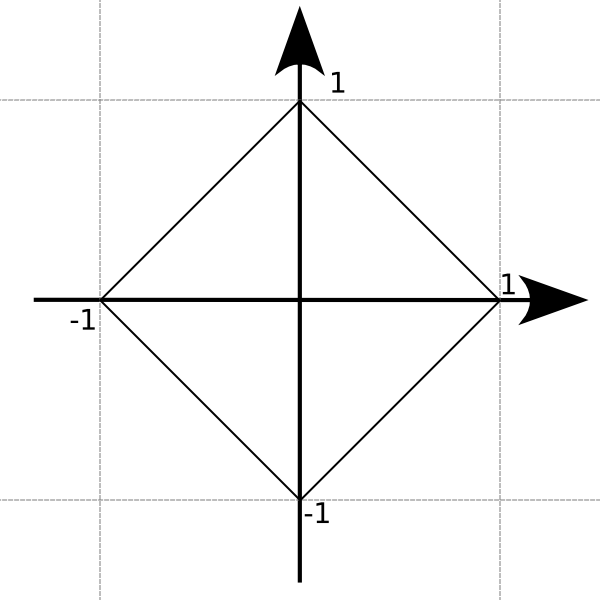
\includegraphics[width=1.0\textwidth]{p_1-kreis.png}
	\caption{$p=1$}
\end{figure}
\begin{figure}[h]
	\centering
	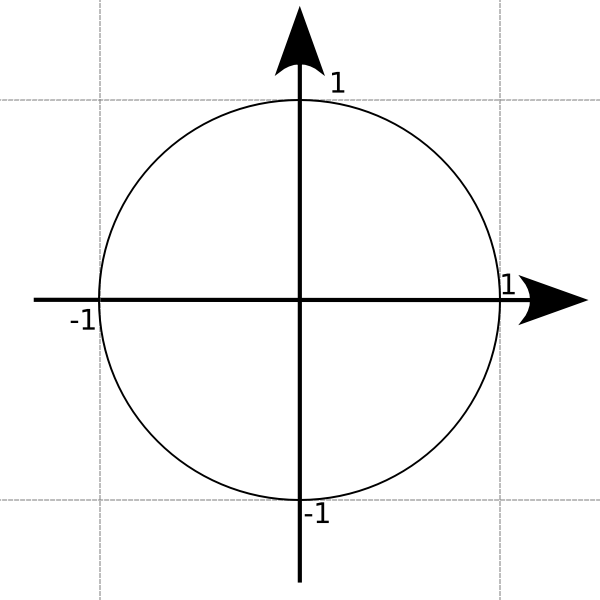
\includegraphics[width=1.0\textwidth]{p_2-kreis.png}
	\caption{$p=2$}
\end{figure}
\begin{figure}[h]
	\centering
	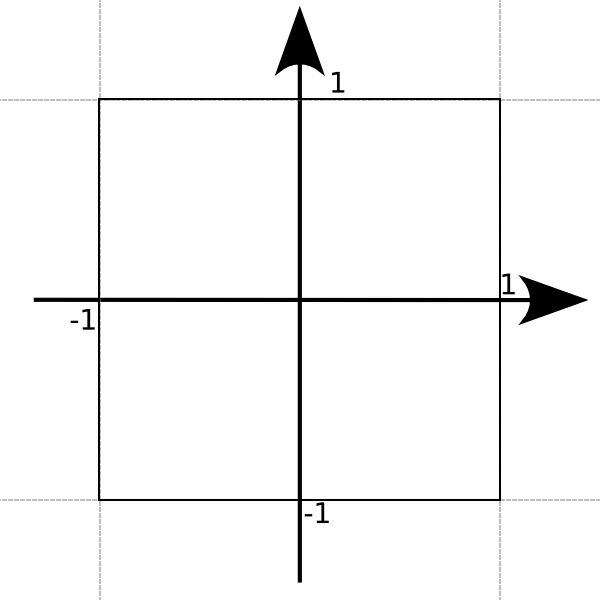
\includegraphics[width=1.0\textwidth]{p_inf-kreis.png}
	\caption{$p=\infty$}
\end{figure}
\clearpage
\newpage

\section*{Aufgabe 2}
Zu zeigen:

$\lim{p\to\infty}{\Vert x \Vert_p}=\Vert x \Vert_\infty$\\
Für ein beliebiges aber festes $x\in\R^n$\\\\
Sei definiert:
\begin{align}
\Vert x \Vert_p &= \sqrt[p]{\sum_{i=1}^n{|x_i|^p}}\\
\Vert x \Vert_\infty &= \max_{i=1,...,n}{|x_i|} 
\end{align}
Wir definieren: 

Sei $|x_k|=\max{|x_1|,...,|x_n|}=\max_{i=1,...,n}{|x_i|} $\\
Wir erhalten folgende Ungleichungsbezihungen:
\begin{align*}
|x_k| &\le \sum_{i=1}^n{|x_i|} &\le n \cdot |x_k|\\
\text{Diese Ungleichung gilt auch für eine Potenz p}\ge 1\\
|x_k|^p &\le \sum_{i=1}^n{|x_i|^p} &\le n \cdot |x_k|^p\\
\text{auch für das Ziehen der p-ten Wurzel bleibt die Ungleichung gültig}\\
\sqrt[p]{|x_k|^p} &\le \sqrt[p]{\sum_{i=1}^n{|x_i|^p}} &\le\sqrt[p]{ n \cdot |x_k|^p}\\
\text{Durch Vereinfachung erhalten wir:}\\
|x_k| &\le \sqrt[p]{\sum_{i=1}^n{|x_i|^p}} &\le\sqrt[p]{ n }\cdot |x_k|
\end{align*}
Wir können nun den Grenzwert bilden.\\
Es folgt:\\
\begin{align*}
\lim_{p\to\infty} |x_k| &\le \lim_{p\to\infty} \sqrt[p]{\sum_{i=1}^n{|x_i|^p}} &\le \lim_{p\to\infty}\sqrt[p]{ n }\cdot |x_k|\\
\text{Wende Produktregel an:}\\
\lim_{p\to\infty} |x_k| &\le \lim_{p\to\infty} \sqrt[p]{\sum_{i=1}^n{|x_i|^p}} &\le \lim_{p\to\infty}\sqrt[p]{ n }\cdot \lim_{p\to\infty}|x_k|\\
\text{Da }|x_k| \text{ konstant ist folgt: } \lim_{p\to\infty} |x_k|=|x_k|\\
|x_k| &\le \lim_{p\to\infty} \sqrt[p]{\sum_{i=1}^n{|x_i|^p}} &\le \lim_{p\to\infty}\sqrt[p]{ n }\cdot |x_k|\\
\text{Für eine Konstante } c \text{ gilt: } \lim_{p\to\infty} \sqrt[p]{c} = 1\\
|x_k| &\le \lim_{p\to\infty} \sqrt[p]{\sum_{i=1}^n{|x_i|^p}} &\le |x_k|\\
\text{Aus *(2) wissen wir, dass }|x_k|=\max_{i=1,...,n}{|x_i|}=\Vert x \Vert_\infty\\
\Vert x \Vert_\infty &\le \lim_{p\to\infty} \sqrt[p]{\sum_{i=1}^n{|x_i|^p}} &\le \Vert x \Vert_\infty\\
\text{Mit Hilfe des Einschnürungssatzes (Sandwichsatz) folgt:}\\
&\lim_{p\to\infty} \sqrt[p]{\sum_{i=1}^n{|x_i|^p}} = \Vert x \Vert_\infty &
\end{align*}\hfill$\square$

\section*{Aufgabe 3}

Sei $(x^k)_{k} \in \mathbb{R}^k, k \in \mathbb{N}$ eine Folge.\\
\\
Sei $x_i = (-1)^i \cdot \frac{1}{\sqrt{i}}$,\\
\\
dann ist:\\
\\
$lim_{n \rightarrow \infty} (x_1)^1 = ||x||_1 = \sum x_i = lim_{n \rightarrow \infty} \sum_{i=1}^{n} (-1)^i \frac{1}{\sqrt{i}} = 0$\\
\\
$lim_{n \rightarrow \infty} (x_2)^2 = ||x||_2 = (\sum (x_i)^2)^{\frac{1}{2}} = lim_{n \rightarrow \infty} (\sum_{i=1}^{n} (-1)^i \frac{1}{i})^{\frac{1}{2}} = \infty$
\end{document}
